\chapter{环面上的极小模型}
我们先前考虑的共形场论都在复平面上。共形场论也可以定义在一般的二维曲面(Riemann面)上。本章讨论环面上极小模型的配分函数,及其模不变性。

\section{圆柱上的CFT}
\begin{figure}[h]
	\centering
	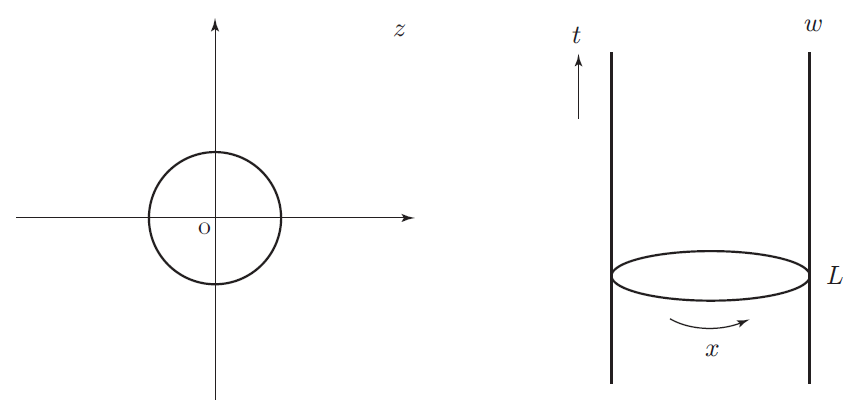
\includegraphics[width=0.6\linewidth]{fig/6.1.png}
	\caption{复平面和圆柱:$z$平面上以原点为圆心的圆,映到$w$平面上固定时刻。}
\end{figure}

考虑周长为 $L $的圆柱上的CFT。时间坐标记作$ t$ ,周向坐标记作 $x$ ,令场 $\phi(t, x) $满足周期性边界条件 $\phi(t, x+L)=\phi(t, x)$ 。坐标$ (t,x)$ 的取值范围是$ -\infty<t<\infty $,$ 0 \leq x \leq L$ 。在有关径向量子化那节(3.3节)解释过,圆柱可通过共形变换映到复平面,如图6.1。复平面上 $z$ 到圆柱上$ w $的共形变换是
\begin{equation}
	w=t+i x=\frac{L}{2 \pi} \log z
\end{equation} 
借助有限共形变换下的变换方程 (3.52) ,可以计算圆柱上CFT中的能动张量 $T_{\mathrm{cyl}}(w)$ 。由
$$
\frac{d w}{d z}=\frac{L}{2 \pi z}, \quad \frac{d^{2} w}{d z^{2}}=\frac{-L}{2 \pi z^{2}}, \quad \frac{d^{3} w}{d z^{3}}=\frac{2 L}{2 \pi z^{3}},
$$
可以得到共形变换 $w=w(z)$ 的Schwarz导数是
$$
S(w, z)=\frac{2-\frac{3}{2}}{z^{2}}=\frac{1}{2 z^{2}}
$$
因此, $z$ 平面上的能动张量$ T(z) $变换为
\begin{equation}
	T_{\text {cyl }}(w)=\left(\frac{2 \pi}{L}\right)^{2}\left(z^{2} T(z)-\frac{c}{24}\right)
\end{equation} 
$c$ 是CFT的中心荷。类似地可得到\footnote{本章考虑$c=\bar{c}$的CFT。如果要求配分函数具有6.3节将讨论的模不变性,可得到$c-\bar{c}$必定是24的整数倍。}
\begin{equation}
	\bar{T}_{\mathrm{cyl}}(\bar{w})=\left(\frac{2 \pi}{L}\right)^{2}\left(\bar{z}^{2} \bar{T}(\bar{z})-\frac{c}{24}\right) 
\end{equation}

圆柱上的Hamiltonian算符$ H $,是时间 $t$ 方向上的演化算符,也是Hamiltonian密度$ T_{t t}(t, x)=T_{\mathrm{cyl}}(w)+\bar{T}_{\mathrm{cyl}}(\bar{w})$ 的空间积分
\begin{equation}
	H=\frac{1}{2 \pi} \int_{0}^{L} T_{t t}(t, x) d x 
\end{equation}
与此类似,圆柱上的动量算符$ P $,是空间 $x$ 方向上的平移算符,也是动量密度 $T_{t x}(t,x)=i\left(T_{\mathrm{cyl}}(w)-\bar{T}_{\mathrm{cyl}}(\bar{w})\right)$ 的空间积分
\begin{equation}
	P=\frac{1}{2 \pi} \int_{0}^{L} \frac{1}{i} T_{t x}(t, x) d x 
\end{equation}
将$ T(z), \bar{T}(\bar{z}) $的模式展开 (3.56) 代入 (6.2),(6.3) ,得到
\begin{align} &T_{\mathrm{cyl}}(w)=\left(\frac{2 \pi}{L}\right)^{2}\left(\sum_{n=-\infty}^{\infty} L_{n} e^{-\frac{2 \pi n}{L}(t+i x)}-\frac{c}{24}\right) \\ &\bar{T}_{\mathrm{cyl}}(\bar{w})=\left(\frac{2 \pi}{L}\right)^{2}\left(\sum_{n=-\infty}^{\infty} \bar{L}_{n} e^{-\frac{2 \pi n}{L}(t-i x)}-\frac{c}{24}\right) \end{align}
作空间积分的话,将只剩下零模$ L_{0}, \bar{L}_{0}$ ,得到Hamiltonian和动量算符是
\begin{align} &H=\frac{2 \pi}{L}\left(L_{0}+\bar{L}_{0}\right)-\frac{\pi c}{6 L}\\ &P=\frac{2 \pi}{L}\left(L_{0}-\bar{L}_{0}\right) \end{align}
共形权为 $(h, \bar{h}) $的初级场$ \phi(z, \bar{z}) $的最高权态 $|h, \bar{h}\rangle $是$ H,P$的本征态,本征值是
\begin{equation}
H=\frac{2 \pi}{L}(h+\bar{h})-\frac{\pi c}{6 L}, \quad P=\frac{2 \pi}{L}(h-\bar{h})
\end{equation} 
$x_{\phi}=h+\bar{h}$ 称为 $\phi $的\textbf{共形维数}, $s=h-\bar{h} $称为 $\phi$ 的\textbf{自旋}。

\section{环面上的CFT}
\subsection{配分函数}
考虑周长 $L $,高 $M$ 的圆柱。在空间和时间方向都要求场 $\phi(t,x)$ 满足周期性边界条件: $\phi(t, x+L)=\phi(t, x)$ , $\phi(t+M, x)=\phi(t, x) $。这个CFT的配分函数是
\begin{equation}
\begin{aligned} Z(L, M) &=\operatorname{Tr} \exp (-M H) \\ &=\operatorname{Tr} \exp \left\{-\frac{2 \pi M}{L}\left(L_{0}+\bar{L}_{0}-\frac{c}{12}\right)\right\} 	
\end{aligned}
\end{equation}
这里的迹是在所考虑CFT的Hilbert空间中取的。

\begin{figure}[h]
	\centering
	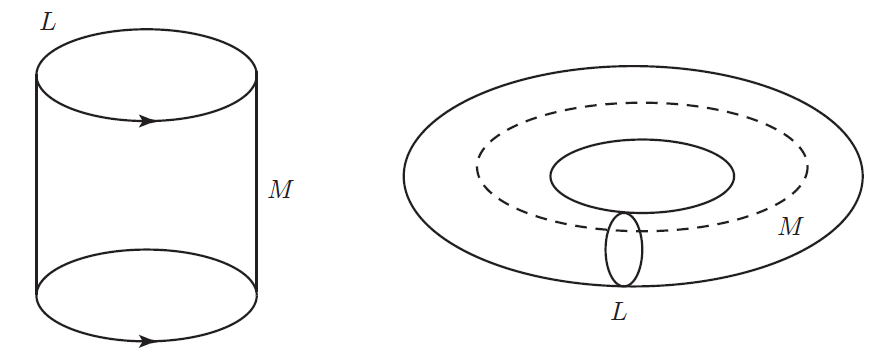
\includegraphics[width=0.6\linewidth]{fig/6.2.png}
	\caption{圆柱和环面:圆柱的上下两端粘起来得到环面。}
\end{figure}

定义CFT的二维曲面是个环面,通过将圆柱的上下两端粘起来得到,如图6.2。环面也可通过取长为 $L,M $的矩形,将左右两端和上下两端粘起来得到,如图6.3。

\begin{figure}[h]
	\centering
	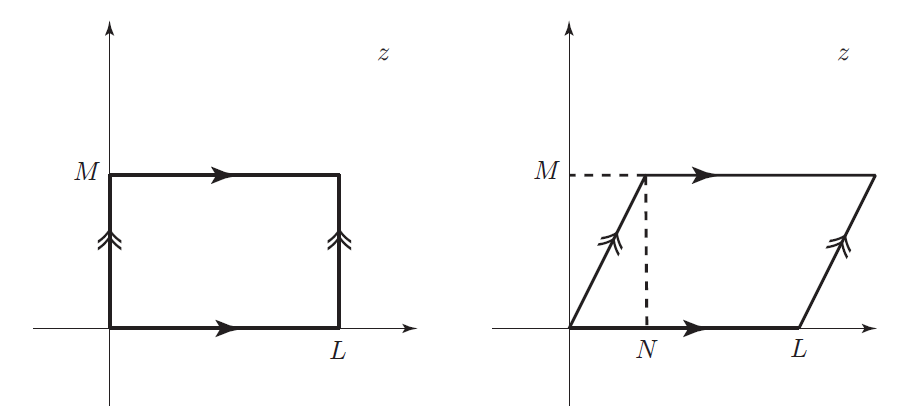
\includegraphics[width=0.6\linewidth]{fig/6.3.png}
	\caption{复平面上的矩形或平行四边形,对边粘起来得到环面。}
\end{figure}

粘起上下两端时,可先令上端转过弧长 $N$ 。这样就在配分函数的迹中,插入了 $x $方向上的平移算符 $\exp (i N P)$ :
\begin{equation}
	\begin{aligned} Z\left(\omega_{1}, \omega_{2}\right) &=\operatorname{Tr} \exp (-M H+i N P) \\ &=\operatorname{Tr} \exp \left\{-\frac{2 \pi M}{L}\left(L_{0}+\bar{L}_{0}-\frac{c}{12}\right)+2 \pi i \frac{N}{L}\left(L_{0}-\bar{L}_{0}\right)\right\} \end{aligned}
\end{equation}
$\omega_{1}=L $,$ \omega_{2}=N+i M$ 是在复平面上表示环面时,描述几何(两顶点的位置)的参数,称为周期。环面可通过将复 z 平面上满足 $z_{1}-z_{2}=n \omega_{1}+m \omega_{2} $( $n,m $是整数)的两点 $z_1,z_2 $视作等价得到。

配分函数可写成
\begin{equation}
	Z(\tau, \bar{\tau})=\operatorname{Tr} q^{L_{0}-\frac{c}{24}} \bar{q}^{\bar{L}_{0}-\frac{c}{24}}
\end{equation} 
其中
\begin{equation}
	q=\exp (2 \pi i \tau), \quad \bar{q}=\exp (-2 \pi i \bar{\tau}), \quad \tau=\frac{\omega_{2}}{\omega_{1}} 
\end{equation}
配分函数依赖于几何参数 $\omega_1,\omega_2 $之比。换句话说,它不依赖于环面的尺寸。复参数$ \tau $称为环面的模参数。

CFT的Hilbert空间可分解成Virasoro代数最高权为 $(h, \bar{h}) $的不可约表示 $V_{h} \otimes \bar{V}_{\bar{h}} $之和。Hilbert空间分解中 $V_{h} \otimes \bar{V}_{\bar{h}}$ 出现的次数记作$ N_{h, \bar{h}} $,那么配分函数可写成
\begin{equation}
	Z(\tau, \bar{\tau})=\sum_{h, \bar{h}} N_{h, \bar{h}} \chi_{(c, h)}(q) \chi_{(c, \bar{h})}(\bar{q})
\end{equation} 
其中
\begin{equation}
	\chi_{(c, h)}(q)=\operatorname{Tr}_{V_{h}} q^{L_{0}-\frac{c}{24}} 
\end{equation}
的迹是在Virasoro代数的不可约表示 $V_h $中取的,称为$ V_h$ 的\textbf{特征标}。类似地,$ \bar{V}_{\bar{h}} $的特征标是
\begin{equation}
	\chi_{(c, \bar{h})}(\bar{q})=\operatorname{Tr}_{\bar{V}_{\bar{h}}} \bar{q}^{\bar{L}_{0}-\frac{c}{24}} 
\end{equation}

\subsection{Virasoro代数的特征标}

Virasoro代数最高权为$ h $的表示 $V_h $中的态由 $L_0 $的本征值标记。级为 $N$ 的态张成的 $V_h$ 的子空间记作 $V_{h, N} $,是 $L_0 $的本征值为 $h+N$ 的本征空间。因为级为 $N$ 的线性独立态的数目等于$ V_{h, N} $的维数 $\operatorname{dim} V_{h, N} $,特征标是
\begin{equation}
	\chi_{(c, h)}(q)=q^{-\frac{c}{24}} \sum_{N=0}^{\infty} \operatorname{dim} V_{h, N} q^{h+N} 
\end{equation}
如果$ V_h$ 不含零模态,也就是说,如果最高权态$ |h\rangle$ 和它的次级态张成的Verma模$ V_h$ 是Virasoro代数的不可约表示,那么级为$ N $的态的数目 $\operatorname{dim} V_{h, N} $,就等于 $N$ 的拆分数 $p(N)$ ,因此特征标是
\begin{equation}
	\chi_{(c, h)}(q)=q^{-\frac{c}{24}} \sum_{N=0}^{\infty} p(N) q^{h+N}=\frac{q^{h-\frac{c}{24}}}{P(q)}
\end{equation} 
其中,$ P(q)=\prod_{n=1}^{\infty}\left(1-q^{n}\right)$ 由 (5.94) 定义。

如果 $V_h$ 含一个级为$ L $的零模态 $|h+L\rangle $,$ V_h $中定义等价关系 $|h+L\rangle=0 $得到的空间 $[h]=V_{h} / V_{h+L}$ 是不可约表示。这时,Verma模 $V_h $的特征标$ \operatorname{Tr}_{V_{h}} q^{L_{0}-\frac{c}{24}}$ ,减去零模态张成的子空间 $V_{h+L} $的特征标$ \operatorname{Tr}_{V_{h+L}} q^{L_{0}-\frac{c}{24}} $,才是不可约表示的特征标
\begin{equation}
\begin{aligned} \chi_{(c, h)}(q) &=q^{-\frac{c}{24}} \sum_{N=0}^{\infty}\left(\operatorname{dim} V_{h, N} q^{h+N}-\operatorname{dim} V_{h+L, N} q^{h+L+N}\right) \\ &=\frac{q^{h-\frac{c}{24}}\left(1-q^{L}\right)}{P(q)} \end{aligned}
\end{equation}

\subsection{极小模型的特征标}

考虑中心荷为$ c=1- 6(p-q)^{2}/(p q) $( $p,q $是互素正整数, $p>q$ )的极小模型的特征标\footnote{不要混淆这里的$q$和模参数$\tau$的函数$q=\exp (2\pi i \tau)$。}\footnote{A. Rocha-Caridi, “Vacuum Vector Representations of the Virasoro Algebra”, in Vertex Operators in Mathematics and Physics, MSRI Publications No.3, Springer, 1984.}。共形权为 $h_{n,m}= [(n p-m q)^{2}-(p-q)^{2}]/(4 p q) $的初级场$ \phi_{(n, m)} $( $0<n<q $,$ 0<m<p$ )对应的最高权表示记作$ \left[h_{n, m}\right] $。5.4节解释过,其中有级为 $nm $的零模态 $\left|h_{q-n, p+m}\right\rangle$和级为 $(q-n)(p-m) $的零模态$ \left|h_{2 q-n, m}\right\rangle $。但[由 (5.29) ]可以发现,Verma模$ V_{h_{q-n, p+m}}$ 和$ V_{h_{2 q-n, m}} $含共同的零模态$ \left|h_{2 q+n, m}\right\rangle $和 $\left|h_{3 q-n, p-m}\right\rangle $,那么从这些态生成的Verma模$ V_{h_{2 q+n, m}} \oplus V_{h_{3 q-n, p-m}} $就有两份。这种零模态无穷嵌套的结构如图6.4。

\begin{figure}[h]
	\centering
	\begin{tikzcd}[column sep=tiny]
		& {h_{n,m}} \arrow[ld] \arrow[rd] &                                           \\
		{h_{2q-n,m}} \arrow[rrd] \arrow[d]  &                                 & {h_{q+n,p-m}} \arrow[lld] \arrow[d]       \\
		{h_{3q-n,p-m}}                      &                                 & {h_{2q+n,m}}                              \\
		\vdots                              &                                 & \vdots                                    \\
		{h_{2qk-n,m}} \arrow[d] \arrow[rrd] &                                 & {h_{(2k-1)q+n,p-m}} \arrow[d] \arrow[lld] \\
		{h_{(2k+1)q-n,p-m}}                 &                                 & {h_{2kq+n,m}}                             \\
		\vdots                              &                                 & \vdots                                   
	\end{tikzcd}
	\caption{最高权表示$[h_{n,m}]$中零模态无穷嵌套的结构。}
\end{figure}

根据这样的结构,最高权表示$ \left[h_{n, m}\right] $的特征标是
\begin{equation}
	\begin{aligned} \chi_{\left(c, h_{n, m}\right)}(\tau)=& \frac{q^{-\frac{c}{24}}}{P(q)}\left\{q^{h_{n, m}}-\sum_{k=1}^{\infty}\left(q^{h_{2 k q-n, m}}+q^{h_{(2 k-1) q+n, p-m}}\right)\right.\\&\left.+\sum_{k=1}^{\infty}\left(q^{h_{(2 k+1) q-n, p-m}}+q^{h_{2 k q+n, m}}\right)\right\} \end{aligned}
\end{equation}
可借助$ h_{n, m}=h_{q-n, p-m}$ 改写成
\begin{equation}
	\begin{aligned} \chi_{\left(c, h_{n, m}\right)}(\tau)=& \frac{q^{-\frac{c}{24}}}{P(q)}\left\{\sum_{k=-\infty}^{\infty}\left(q^{h_{2 k q+n, m}}-q^{h_{2 k q-n, m}}\right)\right\} \\ =&\frac{q^{-\frac{c}{24}}}{P(q)}\left\{\sum_{k=-\infty}^{\infty} \left(q^{\left[(2 k p q+m q-n p)^{2}-(p-q)^{2}\right] /(4 p q)}-q^{\left[(2 k p q+m q+n p)^{2}-(p-q)^{2}\right] /(4 p q)}\right)\right\} \end{aligned}
\end{equation} 

现在来看一些具体的例子。 $(p,q)=(3,2) $时, $c=0 $, $h_{1,1}=0 $的最高权表示只含$ |0\rangle $,因此 $\chi_{\left(c=0, h_{1,1}=0\right)}(q)=1 $。另一方面,代入 (6.22) 给出
\begin{equation}
	\chi_{(0,0)}(q)=\frac{1}{P(q)} \sum_{k=-\infty}^{\infty}(-1)^{k} q^{\frac{3 k^{2}+k}{2}} 
\end{equation}
由此推出
\begin{equation}
	\prod_{n=1}^{\infty}\left(1-q^{n}\right)=\sum_{k=-\infty}^{\infty}(-1)^{k} q^{\frac{3 k^{2}+k}{2}} 
\end{equation}
这可通过在下子节将介绍的Jacobi三重积公式
\begin{equation}
	\prod_{n=1}^{\infty}\left(1-q^{2 n}\right)\left(1-y^{-1} q^{2 n-1}\right)\left(1-y q^{2 n-1}\right)=\sum_{k=-\infty}^{\infty}(-1)^{k} y^{k} q^{k^{2}}
\end{equation} 
中令 $q \rightarrow q^{\frac{3}{2}} $,$ y \rightarrow q^{\frac{1}{2}}$ 得到。

对Ising模型, $(p, q)=(4,3)$ ,有共形权为 $h_{1,1}=0 $,$ h_{1,2}=1/16$ ,$ h_{1,3}=1/2 $的初级场,相应的最高权表示特征标是
\begin{align} &\chi_{\left(\frac{1}{2}, 0\right)}(q)=\frac{q^{-\frac{1}{48}}}{P(q)} \sum_{k=-\infty}^{\infty}\left(q^{\frac{\left[(24 k+1)^{2}-1\right]}{48}}-q^{\frac{\left[(24 k+7)^{2}-1\right]}{48}}\right) \\ &\chi_{\left(\frac{1}{2}, \frac{1}{2}\right)}(q)=\frac{q^{-\frac{1}{48}}}{P(q)} \sum_{k=-\infty}^{\infty}\left(q^{\frac{\left[(24 k+5)^{2}-1\right]}{48}}-q^{\frac{\left[(24 k+11)^{2}-1\right]}{48}}\right) \\ &\chi_{\left(\frac{1}{2}, \frac{1}{16}\right)}(q)=\frac{q^{-\frac{1}{48}}}{P(q)} \sum_{k=-\infty}^{\infty}\left(q^{\frac{\left[(24 k-2)^{2}-1\right]}{48}}-q^{\frac{\left[(24 k+10)^{2}-1\right]}{48}}\right) \end{align}
令 $r=4k $,$ s=4k+1 $, (6.26) 可改写成
\begin{equation}
	\chi_{\left(\frac{1}{2}, 0\right)}(q)=\frac{q^{-\frac{1}{48}}}{P(q)}\left( \sum_{r\equiv 0\ (\text{mod}\ 4)\in \mathbb{Z}} q^{\frac{3 r^{2}+r}{4}}-\sum_{s\equiv 1\ (\text{mod}\ 4)\in \mathbb{Z}} \quad q^{\frac{3 s^{2}+s}{4}}\right)
\end{equation} 
类似地有
\begin{align} &\chi_{\left(\frac{1}{2}, \frac{1}{2}\right)}(q)=\frac{q^{-\frac{1}{48}}}{P(q)}\left( \sum_{r\equiv 1\ (\text{mod}\ 4)\in \mathbb{Z}} q^{\frac{3 r^{2}-r}{4}}-\sum_{s\equiv 2\ (\text{mod}\ 4)\in \mathbb{Z}}q^{\frac{3s^2-s}{4}}\right)\\ &\chi_{\left(\frac{1}{2}, \frac{1}{16}\right)}(q)=\frac{q^{-\frac{1}{48}}}{P(q)} \sum_{k=-\infty}^{\infty}(-1)^{k} q^{3 k^{2}+k} \end{align}
在 (6.24) 中令 $4q\to q^2$ ,可得到
\begin{equation}
	\sum_{k=-\infty}^{\infty}(-1)^{k} q^{3 k^{2}+k}=\prod_{n=1}^{\infty}\left(1-q^{2 n}\right)=P(q) \prod_{n=1}^{\infty}\left(1+q^{n}\right) 
\end{equation}
于是 (6.31) 可写成无穷乘积。至于另两个特征标,考虑线性组合 $\chi_{\left(\frac{1}{2}, 0\right)}(q) \pm \chi_{\left(\frac{1}{2}, \frac{1}{2}\right)}(q)$ ,我们有
\begin{align} &\chi_{\left(\frac{1}{2}, 0\right)}(q)-\chi_{\left(\frac{1}{2}, \frac{1}{2}\right)}(q)=\frac{q^{-\frac{1}{48}}}{P(q)} \sum_{k=-\infty}^{\infty}(-1)^{k} q^{\frac{3 k^{2}+k}{4}} \\ &\chi_{\left(\frac{1}{2}, 0\right)}(q)+\chi_{\left(\frac{1}{2}, \frac{1}{2}\right)}(q)=\frac{q^{-\frac{1}{48}}}{P(q)} \sum_{k=-\infty}^{\infty}(-1)^{\frac{3 k(k+1)}{2}} q^{\frac{3 k^{2}+k}{4}}\end{align}
在Jacobi三重积公式 (6.25) 中令$q \rightarrow q^{\frac{3}{4}} $,$ y \rightarrow q^{\frac{1}{4}} $,可得到
\begin{align} &\sum_{k=-\infty}^{\infty}(-1)^{k} q^{\frac{3 k^{2}+k}{4}}=P(q) \prod_{n=0}^{\infty} (1-q^{n+\frac{1}{2}} ) \\& \sum_{k=-\infty}^{\infty}(-1)^{\frac{3 k(k+1)}{2}} q^{\frac{3 k^{2}+k}{4}}=P(q) \prod_{n=0}^{\infty} (1+q^{n+\frac{1}{2}} ) \end{align}
第二条式子是在第一条式子中令$ q \rightarrow e^{2 \pi i} q $得到的。最终,我们得到了Ising模型特征标的无穷乘积表示:
\begin{align} &\chi_{\left(\frac{1}{2}, 0\right)}(q)=\frac{q^{-\frac{1}{48}}}{2}\left\{\prod_{n=0}^{\infty} (1+q^{n+\frac{1}{2}} )+\prod_{n=0}^{\infty} (1-q^{n+\frac{1}{2}} )\right\} \\ &\chi_{\left(\frac{1}{2}, \frac{1}{2}\right)}(q)=\frac{q^{-\frac{1}{48}}}{2}\left\{\prod_{n=0}^{\infty} (1+q^{n+\frac{1}{2}} )-\prod_{n=0}^{\infty} (1-q^{n+\frac{1}{2}} )\right\} \\ &\chi_{\left(\frac{1}{2}, \frac{1}{16}\right)}(q)=q^{-\frac{1}{48}} \prod_{n=1}^{\infty}\left(1+q^{n}\right) \end{align}
这种无穷乘积表示,对应用自由费米子写的Ising模型CFT。

\subsection{theta函数}

Virasoro代数的特征标可写成模参数 $\tau $的函数$ q=\exp (2 \pi i \tau) $的无穷级数,但其中最基本的结构是Jacobi theta函数$ \vartheta_{a}(z, \tau) $( $a=1,2,3,4 $)。$ z$是复数,$ \tau$ 是满足$ \operatorname{Im} \tau>0 $的复数。本子节用于总结theta函数的基本性质,更详细的讲解见例如\footnote{A. フルヴィッツ,R. クーラント,『楕円関数論』,足立恒雄,小松啓一訳,シュプリンガー・フェ アラーク東京,1991.}\footnote{D. Mumford, Tata Lectures on Theta I, Birkhäuser, 2006.}。
它们的定义是
\begin{align} &\vartheta_{1}(z, \tau)=i \sum_{n=-\infty}^{\infty}(-1)^{n} q^{\frac{1}{2}\left(n-\frac{1}{2}\right)^{2}} e^{i \pi(2 n-1) z} \\ &\vartheta_{2}(z, \tau)=\sum_{n=-\infty}^{\infty} q^{\frac{1}{2}\left(n-\frac{1}{2}\right)^{2}} e^{i \pi(2 n-1) z} \\ &\vartheta_{3}(z, \tau)=\sum_{n=-\infty}^{\infty} q^{\frac{n^{2}}{2}} e^{2 i \pi n z} \\ &\vartheta_{4}(z, \tau)=\sum_{n=-\infty}^{\infty}(-1)^{n} q^{\frac{n^{2}}{2}} e^{2 i \pi n z} \end{align}
只有 $\vartheta_{1}(z, \tau) $是奇函数:
\begin{align} &\vartheta_{1}(-z, \tau)=-\vartheta_{1}(z, \tau) \\ &\vartheta_{a}(-z, \tau)=\vartheta_{a}(z, \tau) \quad(a=2,3,4) \end{align}
特别地,可以看到 $z=0$ 是 $\vartheta_{1}(z, \tau) $的零点。此外,在平移变换 $z \rightarrow z+1/2$ 和 $z \rightarrow z+ \tau/2 $下我们有
\begin{align} &\vartheta_{1}\left(z+\frac{1}{2}, \tau\right)=\vartheta_{2}(z, \tau)\\ &\vartheta_{2}\left(z+\frac{1}{2}, \tau\right)=-\vartheta_{1}(z, \tau)\\ &\vartheta_{3}\left(z+\frac{1}{2}, \tau\right)=\vartheta_{4}(z, \tau)\\ &\vartheta_{4}\left(z+\frac{1}{2}, \tau\right)=\vartheta_{3}(z, \tau) \\ &\vartheta_{1}\left(z+\frac{\tau}{2}, \tau\right)=i q^{\frac{1}{8}} e^{-\pi i z} \vartheta_{4}(z, \tau)\\ &\vartheta_{2}\left(z+\frac{\tau}{2}, \tau\right)=q^{\frac{1}{8}} e^{-\pi i z} \vartheta_{3}(z, \tau)\\ &\vartheta_{3}\left(z+\frac{\tau}{2}, \tau\right)=q^{-\frac{1}{8}} e^{-\pi i z} \vartheta_{2}(z, \tau)\\ &\vartheta_{4}\left(z+\frac{\tau}{2}, \tau\right)=i q^{-\frac{1}{8}} e^{-\pi i z} \vartheta_{1}(z, \tau)  \end{align}
将它们复合起来,得到
\begin{align} &\vartheta_{1}\left(z+\frac{1}{2}+\frac{\tau}{2}, \tau\right)=q^{\frac{1}{8}} e^{-\pi i z} \vartheta_{3}(z, \tau) \\ &\vartheta_{2}\left(z+\frac{1}{2}+\frac{\tau}{2}, \tau\right)=-i q^{\frac{1}{8}} e^{-\pi i z} \vartheta_{4}(z, \tau) \\ &\vartheta_{3}\left(z+\frac{1}{2}+\frac{\tau}{2}, \tau\right)=i q^{-\frac{1}{8}} e^{-\pi i z} \vartheta_{1}(z, \tau) \\ &\vartheta_{4}\left(z+\frac{1}{2}+\frac{\tau}{2}, \tau\right)=q^{-\frac{1}{8}} e^{-\pi i z} \vartheta_{2}(z, \tau) \end{align}
在平移变换$ z \rightarrow z+n+m \tau $下, $\vartheta_{a}(z, \tau) $的值和原来只相差一个数值因子。从 $\vartheta_{a}(z, \tau) $的这一准周期性,可以推出 $\vartheta_{1}(z, \tau)$ 的零点是
$$
z=n+m \tau, \quad n, m \in \mathbb{Z}
$$
$\vartheta_{2}(z, \tau) $, $\vartheta_{3}(z, \tau) $和 $\vartheta_{4}(z, \tau) $的零点,则是 $\vartheta_{1}(z, \tau)$ 的零点分别平移 $1/2$ , $(1+\tau)/2$ 和 $\tau/2 $。引入变量 $y=e^{2 \pi i z} $,那么 $\vartheta_{1}(z, \tau)$ 的零点是 $y=q^{m} $( $m\in \mathbb{Z} $),它有无穷乘积形式
$$
\vartheta_{1}(z, \tau)=2 i C q^{\frac{1}{8}} \sin \pi z \prod_{m=1}^\infty\left(1-y q^{m}\right)\left(1-y^{-1} q^{m}\right)
$$
$C$ 是不依赖于$ z $的数,我们不讨论如何确定 $C$ ,可见\footnote{A. フルヴィッツ,R. クーラント,『楕円関数論』,足立恒雄,小松啓一訳,シュプリンガー・フェ アラーク東京,1991.}。最终的结果是
\begin{align} &\vartheta_{1}(z, \tau)=i 2 e^{\frac{\pi i \tau}{4}} \sin \pi z \prod_{m=1}^{\infty}\left(1-q^{m}\right)\left(1-y q^{m}\right)\left(1-y^{-1} q^{m}\right) \\ &\vartheta_{2}(z, \tau)=2 e^{\frac{\pi i \tau}{4}} \cos \pi z \prod_{m=1}^{\infty}\left(1-q^{m}\right)\left(1+y q^{m}\right)\left(1+y^{-1} q^{m}\right) \\ &\vartheta_{3}(z, \tau)=\prod_{m=1}^{\infty}\left(1-q^{m}\right) (1+y q^{m-\frac{1}{2}} ) (1+y^{-1} q^{m-\frac{1}{2}} ) \\ &\vartheta_{4}(z, \tau)=\prod_{m=1}^{\infty}\left(1-q^{m}\right) (1-y q^{m-\frac{1}{2}}) (1-y^{-1} q^{m-\frac{1}{2}} ) \end{align}
这里, $\vartheta_{4}(z, \tau) $的无穷乘积表示,正是Jacobi三重积公式 (6.25) 中令 $q \rightarrow q^{\frac{1}{2}} $。

接着引入Dedekind eta函数
\begin{equation}
	\eta(\tau)=q^{\frac{1}{24}} P(q)=q^{\frac{1}{24}} \prod_{n=1}^{\infty}\left(1-q^{n}\right), \quad q=e^{2 \pi i \tau}
\end{equation} 
代入 (6.24) 可得到
\begin{equation}
	\eta(\tau)=\sum_{k=-\infty}^{\infty}(-1)^{k} q^{\frac{3}{2}\left(k+\frac{1}{6}\right)^{2}}
\end{equation} 

Ising模型的特征标可用theta和eta函数表示。借助无穷乘积表示
\begin{equation}
	\begin{aligned} \frac{\vartheta_{3}(0, \tau)}{\eta(\tau)} &=\frac{\prod_{m=1}^{\infty}\left(1-q^{m}\right) (1+q^{m-\frac{1}{2}} ) (1+q^{m-\frac{1}{2}} )}{q^{\frac{1}{24}} \prod_{m=1}^{\infty}\left(1-q^{m}\right)} \\ &=q^{-\frac{1}{24}} \prod_{m=1}^{\infty} (1+q^{m-\frac{1}{2}} )^{2} \end{aligned} 
\end{equation}
类似地有
\begin{align} &\frac{\vartheta_{4}(0, \tau)}{\eta(\tau)}=q^{-\frac{1}{24}} \prod_{m=1}^{\infty} (1-q^{m-\frac{1}{2}} )^{2}\\ &\frac{\vartheta_{2}(0, \tau)}{\eta(\tau)}=2 q^{\frac{1}{12}} \prod_{m=0}^{\infty}\left(1+q^{m}\right)^{2}\end{align}
与 (6.37),(6.38),(6.39) 比对可知,
\begin{align} & \chi_{\left(\frac{1}{2}, 0\right)}(q)=\frac{1}{2}\left(\sqrt{\frac{\vartheta_{3}(0, \tau)}{\eta(\tau)}}+\sqrt{\frac{\vartheta_{4}(0, \tau)}{\eta(\tau)}}\right) \\ &\chi_{\left(\frac{1}{2}, \frac{1}{2}\right)}(q)=\frac{1}{2}\left(\sqrt{\frac{\vartheta_{3}(0, \tau)}{\eta(\tau)}}-\sqrt{\frac{\vartheta_{4}(0, \tau)}{\eta(\tau)}}\right) \\ &\chi_{\left(\frac{1}{2}, \frac{1}{16}\right)}(q)=\frac{1}{\sqrt{2}} \sqrt{\frac{\vartheta_{2}(0, \tau)}{\eta(\tau)}} \end{align}
再引入theta函数($ A_1^{(1)} $经典theta函数\footnote{V. G. Kac, Infinite-Dimensional Lie Algebra, 3rd ed., Cambridge Univ. Press, 1990.}\footnote{脇本実,『無限次元リー環』,岩波書店,2008.})
\begin{equation}
	\begin{aligned} &\Theta_{n, m}(z, \tau, u)=e^{2 \pi i m u} \sum_{k=-\infty}^{\infty} e^{2 \pi i m\left(\left(k+\frac{n}{2 m}\right)^{2} \tau+\left(k+\frac{n}{2 m}\right) z\right)}, \\ &n \equiv 0, \cdots, 2 m-1 \quad(\text{mod}\ 2 m) \end{aligned} 
\end{equation}
特别地,为讨论 $(p,q) $极小模型的特征标,我们需要$ u=0$ 情形,因此定义
\begin{equation}
	\begin{aligned} &\Theta_{n, m}(z, \tau)=\sum_{k=-\infty}^{\infty} q^{m\left(k+\frac{n}{2 m}\right)^{2}} e^{2 \pi i m\left(k+\frac{n}{2 m}\right) z} ,\\ &n \equiv 0, \cdots, 2 m-1 \quad(\text{mod}\ 2 m) \end{aligned}
\end{equation}
在 $(p,q) $极小模型的特征标 (6.22) 中代入中心荷$ c=1- 6(p-q)^{2}/(p q)$ ,可得到
\begin{equation}
	\chi_{\left(c, h_{n, m}\right)}(\tau)=K_{\lambda_{n, m}}(\tau)-K_{\lambda_{n,-m}}(\tau) 
\end{equation}
其中
\begin{align} &K_{\lambda}(\tau)=\frac{1}{\eta(\tau)} \Theta_{\lambda, \frac{N}{2}}(0, \tau)\\ & N=2 p q \\ & \lambda_{n, m}=n p-m q  \end{align}

\section{配分函数的模不变性}
因为$ SL(2,\mathbb{Z}) $模变换不改变环面的形状,环面上的配分函数 $Z(\tau, \bar{\tau}) $是模不变的。这对极小模型的结构和四点函数的单值变换不变性施加了很强的限制。为讨论特征标在模变换下的行为,需要进一步的数学基础,我们现在就来解释。

\subsection{ 环面的模变换}

环面可定义为复平面上的二维格。考虑两向量 $\omega_1,\omega_2$ 生成的二维格。假定复数 $\tau=\omega_2/\omega_1 $的虚部为正。$ \tau $称为模参数。环面可通过将复平面上平移 $z \rightarrow z+n \omega_{1}+m \omega_{2}$ ( $n,m$ 是整数)前后的两点视作等价得到。

\begin{figure}[h]
	\centering
	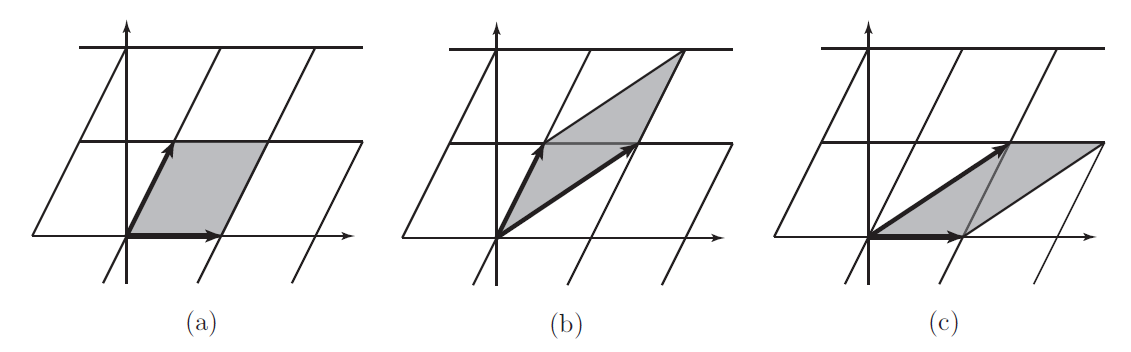
\includegraphics[width=0.6\linewidth]{fig/6.5.png}
	\caption{(a) $(\omega_1,\omega_2)$,(b)$(\omega_1+\omega_2,\omega_2)$,(c) $(\omega_1,\omega_1+\omega_2)$为周期的环面。}
\end{figure}

生成格的基 $(\omega_1,\omega_2) $取法不唯一。例如, $\left(\omega_{1}, \omega_{1}+\omega_{2}\right)$ 和 $\left(\omega_{1}+\omega_{2}, \omega_{2}\right) $也生成同样的格,如图6.5。模参数在这基变换下变为:
\begin{align} &T: \tau \rightarrow \tau+1 \\ &U: \tau \rightarrow \frac{\tau}{\tau+1} \end{align}
定义 $S$ 变换为
\begin{equation}
	S: \tau \rightarrow-\frac{1}{\tau}
\end{equation} 
我们有 $U=T S T $。

考虑一般的基变换
\begin{equation}
	\left(\begin{array}{l} \omega_{2} \\ \omega_{1} \end{array}\right) \rightarrow\left(\begin{array}{l} \omega_{2}^{\prime} \\ \omega_{1}^{\prime} \end{array}\right)=\left(\begin{array}{ll} a & b \\ c & d \end{array}\right)\left(\begin{array}{l} \omega_{2} \\ \omega_{1} \end{array}\right)
\end{equation}
如果前后的两基生成同样的格,那么$ a,b,c,d $要是整数,且 $a d-b c=1 $。换句话说,矩阵
\begin{equation}
	\left(\begin{array}{ll} a & b \\ c & d \end{array}\right) 
\end{equation}
描述的线性变换,要是 $P S L(2, \mathbb{Z})=S L(2, \mathbb{Z}) / \mathbb{Z}_{2} $的元素。模参数在这基变换下变为:
\begin{equation}
	\tau \rightarrow \frac{a \tau+b}{c \tau+d} 
\end{equation}\quad \quad (6.81)
$\mathbb{Z}_2$ 中恒等变换之外的元素,由矩阵
\begin{equation}
	\left(\begin{array}{cc} -1 & 0 \\ 0 & -1 \end{array}\right) 
\end{equation}\quad \quad (6.82)
描述。对模参数来说,它和恒等变换的效果一样。换句话说,矩阵乘上 $-1 $,和原来视作等价。$ P S L(2, \mathbb{Z}) $可由 $T $变换和 $S $变换生成。可以验证矩阵
$$
S=\left(\begin{array}{ll} 0 & -1 \\ 1 & 0 \end{array}\right)
$$
和
$$
T=\left(\begin{array}{ll} 1 & 1 \\ 0 & 1 \end{array}\right)
$$
满足
\begin{equation}
	S^{2}=1, \quad(S T)^{3}=1
\end{equation} \quad \quad (6.83)

\subsection{ Poisson公式}
实数$ x$ 的函数$ f(x)$ 的Fourier变换是
\begin{equation}
	\tilde{f}(y)=\int_{-\infty}^{\infty} e^{-2 \pi i y x} f(x) d x
\end{equation} 
考虑 $f(x) $定义的无穷求和
\begin{equation}
F(x)=\sum_{n=-\infty}^{\infty} f(x+n)	
\end{equation}
$F(x) $具有周期性$ F(x+1)=F(x)$ ,因此可写成Fourier级数
\begin{equation}
	F(x)=\sum_{m=-\infty}^{\infty} F_{m} e^{2 \pi i m x}
\end{equation} 
系数是
\begin{equation}
	F_{m}=\int_{0}^{1} d x e^{-2 \pi i m x} F(x) 
\end{equation}
代入 (6.85) 得到
\begin{equation}
	\begin{aligned} F_{m} &=\sum_{n=-\infty}^{\infty} \int_{0}^{1} e^{-2 \pi i m x} f(x+n) d x \\ &=\sum_{n=-\infty}^{\infty} \int_{n}^{n+1} e^{-2 \pi i m\left(x^{\prime}-n\right)} f\left(x^{\prime}\right) d x^{\prime} \quad\left(令x^{\prime}=x+n \right) \\ &=\int_{-\infty}^{\infty} e^{-2 \pi i m x^{\prime}} f\left(x^{\prime}\right) d x^{\prime} \end{aligned}
\end{equation}
也就是说,Fourier系数$ F_m$ 等于$ f(x) $的Fourier变换 $\tilde{f}(y)$ 在 $y=m $时的值 $\tilde{f}(m)$ 。因此
\begin{equation}
	\sum_{n=-\infty}^{\infty} f(x+n)=\sum_{m=-\infty}^{\infty} \tilde{f}(m) e^{2 \pi i m x}
\end{equation}
令$ x=0 $得到
\begin{equation}
	\sum_{n=-\infty}^{\infty} f(n)=\sum_{m=-\infty}^{\infty} \tilde{f}(m)
\end{equation} 
这称为\textbf{Poisson重求和公式}。

Gauss型函数 $f(x)=e^{-\pi a x^{2}+b x} $的Fourier变换是
\begin{equation}
	\begin{aligned} \tilde{f}(y) &=\int_{-\infty}^{\infty} e^{-2 \pi i y x} e^{-\pi a x^{2}+b x} d x \\ &=\int_{-\infty}^{\infty} e^{-\pi a\left(x+\frac{b-2 \pi i y}{2 \pi a}\right)^{2}-\frac{\pi}{a}\left(y-\frac{b}{2 \pi i}\right)^{2}} d x \\ &=\frac{1}{\sqrt{a}} e^{-\frac{\pi}{a}\left(y-\frac{b}{2 \pi i}\right)^{2}} \end{aligned}
\end{equation} 
于是有
\begin{equation}
	\sum_{n=-\infty}^{\infty} e^{-\pi a n^{2}+b n}=\frac{1}{\sqrt{a}} \sum_{m=-\infty}^{\infty} e^{-\frac{\pi}{a}\left(m-\frac{b}{2 \pi i}\right)^{2}} 
\end{equation}
\subsection{theta函数的模变换}
现在应用Poisson公式,来讨论theta函数在模变换下的行为。模变换由$ T$ 变换和 $S $变换生成,那么考虑这两个变换就够了。

首先讨论Jacobi theta函数在模变换下的行为。 $T $变换 $\tau \rightarrow \tau+1 $下, $q \rightarrow e^{2 \pi i} q $,我们有
\begin{align} &\vartheta_{1}(z, \tau+1)=e^{\frac{\pi i}{4}} \vartheta_{1}(z, \tau)\\ &\vartheta_{2}(z, \tau+1)=e^{\frac{\pi i}{4}} \vartheta_{2}(z, \tau)\\ &\vartheta_{3}(z, \tau+1)=\vartheta_{4}(z, \tau)\\ &\vartheta_{4}(z, \tau+1)=\vartheta_{3}(z, \tau) \end{align}
接着考虑 $S $变换 $\tau\to -1/\tau$ 。在 (6.92) 中,令 $a=-i \tau $, $b=2 \pi i z$ 得到
\begin{equation}
	\sum_{n=-\infty}^{\infty} e^{i \pi \tau n^{2}+2 \pi i z n}=\frac{1}{\sqrt{-i \tau}} e^{-\frac{i z^{2}}{\tau}} \sum_{m=-\infty}^{\infty} e^{i \pi\left(\frac{-1}{\tau}\right) m^{2}+2 \pi i \frac{z}{\tau} m}
\end{equation} 
这就给出 $\vartheta_{3}(z, \tau) $在$ S$ 变换下的行为。其它theta函数同理,结果是
\begin{align} &\vartheta_{1}\left(\frac{z}{\tau}, \frac{-1}{\tau}\right)=-(-i \tau)^{\frac{1}{2}} e^{\frac{i z^{2}}{\tau}} \vartheta_{1}(z, \tau)\\ &\vartheta_{2}\left(\frac{z}{\tau}, \frac{-1}{\tau}\right)=(-i \tau)^{\frac{1}{2}} e^{\frac{i z^{2}}{\tau}} \vartheta_{4}(z, \tau)\\ &\vartheta_{3}\left(\frac{z}{\tau}, \frac{-1}{\tau}\right)=(-i \tau)^{\frac{1}{2}} e^{\frac{i z^{2}}{\tau}} \vartheta_{3}(z, \tau)\\ &\vartheta_{4}\left(\frac{z}{\tau}, \frac{-1}{\tau}\right)=(-i \tau)^{\frac{1}{2}} e^{\frac{i z^{2}}{\tau}} \vartheta_{2}(z, \tau) \end{align}

现在考察Dedekind eta函数。在它的展开式 (6.63) 中代入 $q=e^{2 \pi i \tau}$ ,得到
\begin{equation}
	\eta(\tau)=e^{\frac{\pi i \tau}{12}} \sum_{n=-\infty}^{\infty} e^{3 \pi i \tau n^{2}+\pi i n(\tau+1)}
\end{equation} \quad \quad (6.102)
由此知道 $T $变换$ \tau \rightarrow \tau+1 $给出
\begin{equation}
	\eta(\tau+1)=e^{\frac{\pi i}{12}} \eta(\tau)
\end{equation} 
至于 $S$ 变换,和Jacobi theta函数一样,在 (6.92) 中 $m$ 换成 $-m$ ,令 $a=-3 i \tau $, $b=\pi i(\tau+1)$ ,得到
\begin{equation}
	\begin{aligned} e^{\frac{\pi i \tau}{12}} \sum_{n=-\infty}^{\infty} e^{3 \pi i \tau n^{2}+\pi i n(\tau+1)} &=e^{\frac{\pi i \tau}{12}} \frac{1}{\sqrt{-3 i \tau}} \sum_{m=-\infty}^{\infty} e^{-\frac{\pi}{-3 i \tau}\left(m+\frac{\tau+1}{2}\right)^{2}} \\ &=\frac{e^{\frac{i \pi}{12}\left(\frac{-1}{\tau}\right)} e^{-\frac{i \pi}{6}}}{\sqrt{-3 i \tau}} \sum_{m=-\infty}^{\infty} e^{i \pi\left(\frac{-1}{\tau}\right) \frac{1}{3} m(m+1)} e^{-\frac{i \pi m}{3}} \end{aligned}
\end{equation}
右边$ m $换成$ -m-1$ ,再加上原来的右边取平均,得到
\begin{equation}
	\frac{1}{\sqrt{-3 i \tau}} e^{\frac{i \pi}{12}\left(\frac{-1}{\tau}\right)} \sum_{m=-\infty}^{\infty} e^{i \pi\left(\frac{-1}{\tau}\right) \frac{1}{3} m(m+1)} \cos \frac{\pi(2 m+1)}{6}
\end{equation}
$m=3k,3k\pm 1$ ( $k\in\mathbb{Z}$ )的情形需要分类讨论:
\begin{equation*}
\cos \frac{\pi(2 m+1)}{6}=\left\{\begin{aligned} &\frac{\sqrt{3}}{2}(-1)^{k},&m=3 k, 3 k-1 \\ &0, &m=3 k+1\ \ \ \ \ \ \end{aligned}\right.
\end{equation*}
代入得到
\begin{equation}
	\frac{1}{\sqrt{-i \tau}} e^{\frac{i \pi}{12}\left(\frac{-1}{\tau}\right)} \sum_{k=-\infty}^{\infty}(-1)^{k} e^{i \pi\left(\frac{-1}{\tau}\right)\left(3 k^{2}+k\right)} 
\end{equation}
由此知道$ S$ 变换给出
\begin{equation}
	\eta\left(\frac{-1}{\tau}\right)=(-i \tau)^{\frac{1}{2}} \eta(\tau)
\end{equation} 

最后来考察经典theta函数 (6.71) 。 $T $变换给出
\begin{equation}
	\begin{aligned} \Theta_{n, m}(z, \tau+1) &=\sum_{k=-\infty}^{\infty} e^{2 \pi i m\left(k+\frac{n}{2 m}\right)^{2}} e^{2 \pi i m\left(k+\frac{n}{2 m}\right)^{2} \tau+2 \pi i m\left(k+\frac{n}{2 m}\right) z} \\ &=e^{\frac{\pi i n^{2}}{2 m}} \Theta_{n, m}(z, \tau) \end{aligned}
\end{equation}
至于 $S$ 变换,仿照Jacobi theta函数。定义给出
\begin{equation}
	\Theta_{n, m}\left(\frac{z}{\tau},-\frac{1}{\tau}\right)=\sum_{k=-\infty}^{\infty} e^{2 \pi i m\left(k+\frac{n}{2 m}\right)^{2}\left(-\frac{1}{\tau}\right)+2 \pi i m\left(k+\frac{n}{2 m}\right) \frac{z}{\tau}} 
\end{equation}
在 (6.92) 中, $m $换成$ -l$ ,令 $a=(2im)/\tau $, $b=-2\pi i m(n/m-z)k/\tau$ ,得到右边是
\begin{equation}
e^{2 \pi i m\left(\frac{n^{2}}{4 m^2}\left(-\frac{1}{\tau}\right)+\frac{n z}{2 m \tau}\right)} \sqrt{\frac{1}{\frac{2 i m}{\tau}}} \sum_{l=-\infty}^{\infty} e^{\frac{i \pi \tau}{2 m}\left(l-\frac{n-z m}{\tau}\right)^{2}}
\end{equation} 
指数上的表达式和原来的theta函数不太一样,但整数 $l$ 除以 $2m $提出余数,即写成 $l=l^{\prime} 2 m+n^{\prime}$ ( $l^{\prime} \in \mathbb{Z}, n^{\prime}=0, \cdots, 2 m-1 $)后,我们有
\begin{equation}
	\begin{aligned} \frac{i \pi \tau}{2 m}\left(l-\frac{n-z m}{\tau}\right)^{2}=& 2 \pi i m\left(\left(l^{\prime}+\frac{n^{\prime}}{2 m}\right)^{2}\tau+\left(l^{\prime}+\frac{n^{\prime}}{2 m}\right) z\right) \\ &-2 \pi i l^{\prime} n-\frac{i \pi n^{\prime} n}{m}+\frac{i \pi }{2 m \tau}(n-z m)^{2} \end{aligned}
\end{equation}
代入 (6.110) 整理,得到$ S $变换给出
\begin{equation}
	\Theta_{n, m}\left(\frac{z}{\tau},-\frac{1}{\tau}\right)=\frac{(-i \tau)^{\frac{1}{2}}}{(2 m)^{\frac{1}{2}}} e^{\frac{\pi i m z^{2}}{2\tau}} \sum_{n^{\prime}=0}^{2 m-1} e^{-\frac{i \pi n n^{\prime}}{m}} \Theta_{n^{\prime}, m}(z, \tau)
\end{equation} 

\subsection{Virasoro特征标的模变换}
基于上子节的结果,我们来讨论中心荷为$ c=1- 6(p-q)^{2} /(p q) $的极小模型中退化表示 $\left[h_{n, m}\right] $的特征标 $\chi_{n, m}(\tau) $在模变换下的行为。

首先,以Ising模型为例。我们对Jacobi theta和Dedekind eta函数表示的特征标 (6.67),(6.68),(6.69) 作模变换。在 $T$ 变换下, (6.93)-(6.96) 中令 $z=0$ ,结合 (6.103) 得到
\begin{align} &\chi_{\left(\frac{1}{2}, 0\right)}(\tau+1)=e^{-\frac{i \pi}{24}} \chi_{\left(\frac{1}{2}, 0\right)}(\tau)\\ &\chi_{\left(\frac{1}{2}, \frac{1}{2}\right)}(\tau+1)=-e^{-\frac{i \pi}{24}} \chi_{\left(\frac{1}{2}, \frac{1}{2}\right)}(\tau) \\ & \chi_{\left(\frac{1}{2}, \frac{1}{16}\right)}(\tau+1)=e^{\frac{i \pi}{24}} \chi_{\left(\frac{1}{2}, \frac{1}{16}\right)}(\tau)  \end{align}
在 $S $变换下, (6.98)-(6.101) 中令 $z=0$ ,结合 (6.107) 得到
\begin{align} &\chi_{\left(\frac{1}{2}, 0\right)}\left(-\frac{1}{\tau}\right)=\frac{1}{2}\left(\sqrt{\frac{\vartheta_{3}(0, \tau)}{\eta(\tau)}}+\sqrt{\frac{\vartheta_{2}(0, \tau)}{\eta(\tau)}}\right) \\ &\chi_{\left(\frac{1}{2}, \frac{1}{2}\right)}\left(-\frac{1}{\tau}\right)=\frac{1}{2}\left(\sqrt{\frac{\vartheta_{3}(0, \tau)}{\eta(\tau)}}-\sqrt{\frac{\vartheta_{2}(0, \tau)}{\eta(\tau)}}\right)\\ &\chi_{\left(\frac{1}{2}, \frac{1}{16}\right)}\left(-\frac{1}{\tau}\right)=\frac{1}{\sqrt{2}} \sqrt{\frac{\vartheta_{4}(0, \tau)}{\eta(\tau)}} \end{align}
用原来的特征标写是
\begin{equation}
	\begin{aligned} &\chi_{\left(\frac{1}{2}, 0\right)}\left(-\frac{1}{\tau}\right)=\frac{1}{2} \chi_{\left(\frac{1}{2}, 0\right)}(\tau)+\frac{1}{2} \chi_{\left(\frac{1}{2}, \frac{1}{2}\right)}(\tau)+\frac{\sqrt{2}}{2} \chi_{\left(\frac{1}{2}, \frac{1}{16}\right)}(\tau)\\ &\chi_{\left(\frac{1}{2}, \frac{1}{2}\right)}\left(-\frac{1}{\tau}\right)=\frac{1}{2} \chi_{\left(\frac{1}{2}, 0\right)}(\tau)+\frac{1}{2} \chi_{\left(\frac{1}{2}, \frac{1}{2}\right)}(\tau)-\frac{\sqrt{2}}{2} \chi_{\left(\frac{1}{2}, \frac{1}{16}\right)}(\tau) \\ &\chi_{\left(\frac{1}{2}, \frac{1}{16}\right)}\left(-\frac{1}{\tau}\right)=\frac{\sqrt{2}}{2} \chi_{\left(\frac{1}{2}, 0\right)}(\tau)-\frac{\sqrt{2}}{2} \chi_{\left(\frac{1}{2}, \frac{1}{2}\right)}(\tau) \end{aligned}
\end{equation}
我们看到,模变换造成了特征标间的变换。那么,一般的极小模型是什么样呢?

对 $(p,q)$ 极小模型,基于特征标的定义 (6.22) 考虑$ T $变换。在 $T $变换 $\tau \rightarrow \tau+1$ 下,$ q=e^{2\pi i \tau} \rightarrow q e^{2 \pi i}$ 。 (6.22) 中的 $h_{2 k q+n, m} $, $h_{2 k q-n, m} $都在Verma模 $V_{h_{n, m}} $中,因此都是 $h_{n, m}$ 加上一整数,那么特征标只是乘上一个相位因子:
\begin{equation}
	\chi_{\left(c, h_{n, m}\right)}(\tau+1)=e^{2 \pi i\left(h_{n, m}-\frac{c}{24}\right)} \chi_{\left(c, h_{n, m}\right)}(\tau)
\end{equation} 
根据eta和经典theta函数在 $T $变换下的行为 (6.103),(6.108) ,也能看到这点。我们考察$ K_{\lambda}(\tau) $(6.73) ,$ T $变换给出
\begin{equation}
	K_{\lambda}(\tau+1)=e^{2 \pi i\left(\frac{\lambda^{2}}{2 N}-\frac{1}{24}\right)} K_{\lambda}(\tau)
\end{equation}
在 $K_\lambda $表示的特征标 (6.72) 中,第一项乘上相位因子 $\exp \left(2 \pi i\left(\frac{\lambda_{n, m}^{2}}{2 N}-\frac{1}{24}\right)\right)$ ,第二项乘上相位因子 $\exp \left(2 \pi i\left(\frac{\lambda_{n,-m}^{2}}{2 N}-\frac{1}{24}\right)\right) $,两相位之差是
$$
\frac{\pi i \lambda_{n, m}^{2}}{N}-\frac{\pi i \lambda_{n,-m}^{2}}{N}=2 m n \pi i
$$
因此给出同样的贡献,我们有
$$
\chi_{\left(c, h_{n, m}\right)}(\tau+1)=e^{\pi i\left(\frac{\lambda_{n, m}^{2}}{N}-\frac{1}{12}\right)} \chi_{\left(c, h_{n, m}\right)}(\tau)
$$
因为
$$
h_{n, m}-\frac{c}{24}=\frac{(n p-m q)^{2}}{4 p q}-\frac{1}{24}
$$
这同 (6.120) 一样。

接着考虑$ S $变换。根据eta和经典theta函数的变换行为 (6.107),(6.112) ,我们有
\begin{equation}
K_{\lambda}\left(-\frac{1}{\tau}\right)=\frac{1}{\sqrt{N}} \sum_{m=0}^{N-1} e^{-\frac{2 \pi i \lambda m}{N}} K_{m}(\tau)
\end{equation} 
要由此得到特征标在 $S$变换下的行为,关注 $K_{\lambda}(\tau) $的对称性至关重要。首先,从经典theta函数的定义可以看到
\begin{equation}
	K_{\lambda+N}(\tau)=K_{-\lambda}(\tau)=K_{\lambda}(\tau)
\end{equation} 
也就是说, $\tau $固定时$ K_{\lambda}(\tau) $只与 $\lambda\ \text{mod} \ N$ 有关,与 $\lambda $的符号也无关。

然后,因为 $p,q$ ( $p<q$ )是互素正整数,存在整数 $n_0,m_0 $使得
\begin{equation}
n_{0} p-m_{0} q=1	
\end{equation}
定义整数
\begin{equation}
	\omega_{0} \equiv n_{0} p+m_{0} q \quad(\text{mod}\ N)
\end{equation}
我们有
\begin{equation}
	\begin{aligned} \omega_{0} \lambda_{n, m} & \equiv\left(n_{0} p+m_{0} q\right)(n p-m q) \\ &=\left(n_{0} p-m_{0} q\right)(n p +m q)+\left(n m_{0}-n_{0} m\right) 2 p q \\ & \equiv \lambda_{n,-m} \quad(\text{mod} \ N) \end{aligned} 
\end{equation}
换句话说,$ \lambda_{n, m} $乘上$ \omega_0 $相当于改变 $m$ 的符号,此外$ \omega_{0}^{2} \equiv 1\ (\text{mod}\ N) $。因此可以定义
\begin{equation}
	\chi_{\lambda}(\tau)=K_{\lambda}(\tau)-K_{\omega_{0} \lambda}(\tau)
\end{equation} 
这样的话,
\begin{equation}
	\chi_{\left(c, h_{n, m}\right)}(\tau)=\chi_{\lambda_{n, m}}(\tau) 
\end{equation}
它满足
\begin{equation}
	\chi_{\lambda+N}(\tau)=\chi_{-\lambda}(\tau)=-\chi_{\omega_{0} \lambda}(\tau)=\chi_{\lambda}(\tau) 
\end{equation}
根据$ K_{\lambda}(\tau) $在$ S $变换下的行为,我们有
\begin{equation}
	\chi_{\lambda}\left(-\frac{1}{\tau}\right)=\frac{1}{\sqrt{N}} \sum_{n^{\prime}=0}^{N-1}\left(e^{-\frac{i 2 \pi \lambda n^{\prime}}{N}} K_{n^{\prime}}(\tau)-e^{-\frac{i 2 \pi \omega_{0} \lambda n^{\prime}}{N}} K_{n^{\prime}}(\tau)\right)
\end{equation} 
右边第二项对$ n'$ 的求和,可换成对$ \omega_0n' $的求和,于是右边可改写成
$$
\frac{1}{\sqrt{N}} \sum_{n^{\prime}=0}^{N-1} e^{-\frac{i 2 \pi \lambda n^{\prime}}{N}}\left(K_{n^{\prime}}(\tau)-K_{\omega_{0} n^{\prime}}(\tau)\right)
$$
我们得到 $S $变换给出
\begin{equation}
	\chi_{\lambda}\left(-\frac{1}{\tau}\right)=\frac{1}{\sqrt{N}} \sum_{n^{\prime}=0}^{N-1} e^{-\frac{i 2 \pi \lambda n^{\prime}}{N}} \chi_{n^{\prime}}(\tau)
\end{equation} 
注意,即使我们令$ \lambda=\lambda_{n, m} $,右边的特征标也不直接对应退化初级场。(6.124) 两边同乘 $n' $,得到 $n^{\prime}=a p-b q$ ( $a,b $是整数)。$ n' $满足$ \omega_{0} n^{\prime} \equiv \pm n^{\prime}\ (\text{mod}\ N)$ 时,[由 (6.129) ] $\chi_{n^{\prime}}(\tau) =0 $,不贡献求和。[由 (6.126) ]这个条件等价于
$$
a p+b q \equiv \pm(a p-b q) \quad(\text{mod}\ N)
$$
取正号的话,这又等价于$ b $是 $p$ 的倍数,于是 $n'$ 是 $p$ 的倍数。取负号的话,这又等价于 $a$ 是 $q $的倍数,于是$ n'$ 是 $q $的倍数。反过来,如果 $n' $是$ p$ 或 $q$ 的倍数,显然就满足 $\omega_{0} n^{\prime} \equiv \pm n^{\prime}$ 。总结一下, (6.131) 中$ n'$ 是$ p$ 或 $q $的倍数时不贡献求和。在 $0, \cdots, 2 p q-1 $中,这样的 $n' $共有 $2p+2q-2 $个( $0$ 和 $p q $重复了),去掉这些还剩下$2 p q-(2 p+2 q-2)=2(p-1)(q-1) $个。

在剩下的 $n'$ 中,我们找对应Virasoro代数退化表示的,也就是整数对$(a,b) $等于$ (n,m) $的。$ n,m$ 的范围是$ 1 \leq n \leq q-1$ ,$ 1 \leq m \leq p-1$ ,但5.4节讨论过,初级场 $\phi_{(n, m)}$ 和 $\phi_{(q-n, p-m)} $等价。 $(m,n) $等价关系的代表元可选成使得
\begin{equation}
	n p>m q
\end{equation} 
成立。对应这些独立初级场的 $(n,m) $的集合记作 $E_{p, q} $。这样的初级场共有 $(p-1)(q-1) / 2 $个。
对这些代表元$ (n,m)$ ,$ \lambda_{n, m}=n p-m q $,$ \omega_{0} \lambda_{n, m} \equiv \lambda_{n,-m}$ ,$ N-\lambda_{n,m}\equiv \lambda_{q-n,p-m} $,$ \omega_0(N-\lambda_{n,m})\equiv \lambda_{q-n,m-p} $都不相等。等于它们的 $n' $共有$ (p-1)(q-1) / 2 \times 4=2(p-1)(q-1) $个,这正是上面计算的不是 $p $或 $q$ 倍数的 $n'$ 的数目。

那么,求和 (6.131) 用属于$ E_{p, q}$ 的整数对写是\footnote{结合 (6.129)}
\begin{equation}
	\begin{aligned} \chi_{\lambda}\left(-\frac{1}{\tau}\right)=& \frac{1}{\sqrt{N}} \sum_{(n, m) \in E_{p, q}}\left(e^{\frac{2 \pi i \lambda \lambda_{n, m}}{N}}-e^{\frac{2 \pi i \lambda \omega_{0} \lambda_{n, m}}{N}}\right.\\&\left.+e^{\frac{2 \pi i \lambda\left(N-\lambda_{n, m}\right)}{N}}-e^{\frac{2 \pi i \lambda \omega_{0}\left(N-\lambda_{n, m}\right)}{N}}\right) \chi_{\lambda_{n, m}}(\tau) \end{aligned} 
\end{equation}
右边括号中的因子可改写成
\begin{equation}
	2 \cos \left(\frac{2 \pi \lambda \lambda_{n, m}}{N}\right)-2 \cos \left(\frac{2 \pi \lambda \lambda_{n,-m}}{N}\right)=4 \sin \left(\frac{\pi \lambda n}{q}\right) \sin \left(\frac{\pi \lambda m}{p}\right)
\end{equation} 
令$ \lambda=\lambda_{n', m'} $,我们得到$ S $变换给出
\begin{equation}
	\begin{aligned} \chi_{\lambda_{n^{\prime}, m^{\prime}}}\left(-\frac{1}{\tau}\right)=& \frac{1}{\sqrt{N}} \sum_{(n, m) \in E_{p, q}} 4 \sin \left(\frac{\pi\left(n^{\prime} p-m^{\prime} q\right) n}{q}\right) \\ & \times \sin \left(\frac{\pi\left(n^{\prime} p-m^{\prime} q\right) m}{p}\right) \chi_{\lambda_{n, m}}(\tau) \end{aligned} 
\end{equation}

总结一下,Virasoro代数的特征标$ \chi_{\left(c, h_{n, m}\right)}(\tau)$ 在 $T,S $变换下,变为
\begin{align} &\chi_{\left(c, h_{n, m}\right)}(\tau+1)=e^{2 \pi i\left(h_{n, m}-\frac{c}{24}\right)} \chi_{\left(c, h_{n, m}\right)}(\tau) \\ &\chi_{\left(c, h_{n, m}\right)}\left(-\frac{1}{\tau}\right)=\sum_{\left(n^{\prime}, m^{\prime}\right) \in E_{p, q}} S_{n, m}^{n^{\prime}, m^{\prime}} \chi_{\left(c, h_{n^{\prime}, m^{\prime}}\right)}(\tau) \end{align}
其中
\begin{equation}
	S_{n, m}^{n^{\prime}, m^{\prime}}=\left(\frac{8}{p q}\right)^{\frac{1}{2}}(-1)^{1+n m^{\prime}+m n^{\prime}} \sin \frac{\pi n n^{\prime} p}{q} \sin \frac{\pi m m^{\prime} q}{p} 
\end{equation}
称为\textbf{模 $S $矩阵}。

在Ising模型的情形,$ (p, q)=(3,4)$ ,$ E_{3,4}=\{(2,1),(3,1),(3,2)\}$ ,可由上式算出模 $S$ 矩阵是
\begin{equation}
	\left(\begin{array}{rrr} S_{3,2}^{3,2} & S_{3,2}^{3,1} & S_{3,2}^{2,1} \\ S_{3,1}^{3,2} & S_{3,1}^{3,1} & S_{3,1}^{2,1} \\ S_{2,1}^{3,2} & S_{2,1}^{3,1} & S_{2,1}^{2,1} \end{array}\right)=\left(\begin{array}{ccc} \frac{1}{2} & \frac{1}{2} & \frac{1}{\sqrt{2}} \\ \frac{1}{2} & \frac{1}{2} & -\frac{1}{\sqrt{2}} \\ \frac{1}{\sqrt{2}} & -\frac{1}{\sqrt{2}} & 0 \end{array}\right)
\end{equation} 
确实与 (6.119) 一致。

模 $S$ 矩阵 (6.138) 是实对称矩阵,满足$ S^{2}=1$ 。可从 (6.131) 推出
\begin{equation}
	\sum_{\left(n^{\prime}, m^{\prime}\right) \in E_{p, q}} S_{n, m}^{n^{\prime}, m^{\prime}} S_{n^{\prime}, m^{\prime}}^{n^{\prime \prime}, m^{\prime \prime}}=\frac{1}{N} \sum_{\mu=0}^{N-1} e^{\frac{2 \pi i\left(\lambda_{n, m}+\lambda_{n^{\prime \prime}, m^{\prime \prime}}\right) \mu}{N}} 
\end{equation})
右边在
\begin{equation}
	\lambda_{n, m}+\lambda_{n^{\prime \prime}, m^{\prime \prime}} \equiv 0 \quad(\text{mod}\ N)
\end{equation}
时等于 1 ,其它情形等于 0 。 $(n, m),\left(n^{\prime \prime}, m^{\prime \prime}\right) $属于$ E_{p, q} $时,上式等价于 $n^{\prime \prime}=q-n $,$ m^{\prime \prime}=p-m $,由此知道在$ E_{p, q} $中矩阵 $S^{2}=1 $。

\subsection{ADE分类}
上子节推导了Virasoro代数特征标在模变换下的行为。 $(p,q) $极小模型的配分函数由正反全纯部分的特征标组成:
\begin{equation}
	Z(\tau, \bar{\tau})=\sum_{(n, m),\left(n^{\prime}, m^{\prime}\right) \in E_{p, q}} N_{n, m, n^{\prime}, m^{\prime}} \chi_{\left(c, h_{n, m}\right)}(\tau) \overline{\chi_{\left(c, \bar{h}_{n^{\prime}, m^{\prime}}\right)}(\tau)} 
\end{equation}
这里, $N_{n, m, n^{\prime}, m^{\prime}} $指共形权 $h_{n, m}, \bar{h}_{n^{\prime}, m^{\prime}} $出现的次数,是非负整数。如果
\begin{equation}
	N_{n, m, n^{\prime}, m^{\prime}}=\delta_{n, n^{\prime}} \delta_{m, m^{\prime}}
\end{equation} 
从 S 是对称矩阵和 $S^{2}=1 $可以推出,配分函数是模不变的。 $T$ 变换下不变是显然的。 (6.143) 成立的配分函数称为\textbf{对角不变配分函数}。

Cappelli-Itzykson-Zuber\footnote{A. Cappelli, C. Itzykson and J. B. Zuber, Nucl. Phys. B 280 (1987) 445.}对 $(p,q) $极小模型模不变配分函数的分类进行了猜测,之后加藤\footnote{A. Kato, Mod. Phys. Lett. A 2 (1987) 585.}和Cappelli-Itzykson-Zuber\footnote{A. Cappelli, C. Itzykson and J. B. Zuber, Commun. Math. Phys. 113 (1987) 1.}实现了证明。这个分类可同Lie代数的ADE分类对应起来,结果列在表6.1中。
\begin{table}[h]
	\centering
	\begin{tabular}{|c|c|}
		\hline$\left(A_{q-1}, A_{p-1}\right)$ & $\frac{1}{2} \sum_{n=1}^{q-1} \sum_{m=1}^{p-1}\left|\chi_{n, m}\right|^2$ \\
		\hline$\left(D_{2 \rho+2}, A_{p-1}\right)$ & $\frac{1}{2} \sum_{m=1}^{p-1}\left(\sum_{\substack{n=1, \text { odd } \\
				n \neq 2 \rho+1}}^{4 \rho+1}\left|\chi_{n, m}\right|^2+2\left|\chi_{2 \rho+1, m}\right|^2\right.$ \\
		$q=4 \rho+2, \rho \geq 1$ & $\left.+\sum_{n=1, \text { odd }}^{2 \rho-1}\left(\chi_{n, m} \overline{\chi_{4 \rho+2-n, m}}+\overline{\chi_{n, m}} \chi_{4 \rho+2-n, m}\right)\right)$ \\
		\hline$\left(D_{2 \rho+1}, A_{p-1}\right)$ & $\frac{1}{2} \sum_{m=1}^{p-1}\left(\sum_{n=1, \text { odd }}^{4 \rho-1}\left|\chi_{n, m}\right|^2+\left|\chi_{2 \rho, m}\right|^2\right.$ \\
		$q=4 \rho, \rho \geq 2$ & $\left.+\sum_{n=2, \text { even }}^{2 \rho-2}\left(\overline{\chi_{n, m}} \chi_{4 \rho-n, m}+\overline{\chi 4 \rho-n, m} \chi_{n, m}\right)\right)$ \\
		\hline$\left(E_6, A_{p-1}\right) q=12$ & $\frac{1}{2} \sum_{m=1}^{p-1}\left\{\left|\chi_{1, m}+\chi_{7, m}\right|^2+\left|\chi_{4, m}+\chi_{8, m}\right|^2+\left|\chi_{5, m}+\chi_{11, m}\right|^2\right\}$ \\
		\hline$\left(E_7, A_{p-1}\right) q=18$ & \begin{tabular}{l}
			$\frac{1}{2} \sum_{m=1}^{p-1}\left\{\left|\chi_{1, m}+\chi_{17, m}\right|^2+\left|\chi_{5, m}+\chi_{13, m}\right|^2+\left|\chi_{7, m}+\chi_{11, m}\right|^2\right.$ \\
			$\left.\quad+\left|\chi_{9, m}\right|^2+\left[\overline{\left(\chi_{3, m}+\chi_{15, m}\right)} \chi_{9, m}+\overline{\chi_{9, m}}\left(\chi_{3, m}+\chi_{15, m}\right)\right]\right\}$
		\end{tabular} \\
		\hline$\left(E_8, A_{p-1}\right) q=30$ & \begin{tabular}{l}
			$\frac{1}{2} \sum_{m=1}^{p-1}\left\{\left|\chi_{1, m}+\chi_{11, m}+\chi_{19, m}+\chi_{29, m}\right|^2\right.$ \\
			$\left.\quad+\left|\chi_{7, m}+\chi_{13, m}+\chi_{17, m}+\chi_{23, m}\right|^2\right\}$
		\end{tabular} \\
		\hline
	\end{tabular}
	\caption{模不变配分函数的分类。在Lie代数的分类中,Dynkin图中节点间总是只有一条线的称为simply-laced Lie代数,也就是ADE型Lie代数。除了典型Lie代数$A_n=\mathfrak{su}(n+1)$和$D_n=\mathfrak{so}(2n)$,还有例外Lie代数$E_6$,$E_7$,$E_8$。求和中出现的自然数正是各Lie代数的指数。}
\end{table}

\section{模不变性的应用}
本节讨论配分函数的模不变性对CFT结构施加的限制。带一般中心荷$ c$ 的CFT的配分函数由Virasoro代数的特征标组成:
\begin{equation}
	Z(\tau, \bar{\tau})=\sum_{h, \bar{h}} N_{h, \bar{h}} \chi_{(c, h)}(\tau) \chi_{(c, \bar{h})}(\bar{\tau}) 
\end{equation}\quad \quad (6.144)
这里是对初级场的共形权 $(h, \bar{h}) $求和, $N_{h, \bar{h}}$ 是相应初级场在理论中出现的次数。特征标 $\chi_{(c, h)}(\tau) $可写成$ q=e^{2 \pi i \tau} $的级数
\begin{equation}
	\chi_{(c, h)}(\tau)=\sum_{n=0}^{\infty} d_{h}(n) q^{n+h-\frac{c}{24}}
\end{equation} 
这里, $d_{h}(n) $是最高权表示 $[h]$ 中级为$n $的态的数目。

令模参数是纯虚数 $\tau=i \delta$ ( $\delta>0 $),那么$ q=e^{-2 \pi \delta}$ 是实数,取值范围 $0<q<1 $。在退化表示中,我们将零模态视作同零等价,态的数目也就相应地减少。因此,$ d_{h}(n)$ 不超过Verma模中态的数目$ P(n) $,我们有不等式
\begin{equation}
	\chi_{(c, h)}(\tau) \leq q^{h-\frac{c}{24}} \sum_{n=0}^{\infty} P(n) q^{n}=q^{-\frac{c-1}{24}+h} \eta^{-1}(\tau)
\end{equation} 
在模变换$ \tau \rightarrow- 1/\tau=i/\delta$ 下,eta函数的变换行为给出
\begin{equation}
	\eta(\tau)=\frac{1}{(\operatorname{Im} \tau)^{1 / 2}} \eta\left(-\frac{1}{\tau}\right)
\end{equation} 
其中
\begin{equation}
	\eta\left(-\frac{1}{\tau}\right)=\tilde{q}^{\frac{1}{24}} \prod_{n=1}^{\infty}\left(1-\tilde{q}^{n}\right), \quad \tilde{q}=e^{-\frac{2 \pi i}{\tau}}=e^{-\frac{2 \pi}{\delta}}
\end{equation}
现在考察 (6.146) 右边在 $\operatorname{Im} \tau=\delta \rightarrow 0 $时的行为。这时
\begin{equation}
	q=e^{-2 \pi \delta} \rightarrow 1
\end{equation}
那么
\begin{equation}
	\tilde{q}=e^{-\frac{2 \pi}{\delta}} \rightarrow 0 
\end{equation}
由 (6.147) 知
\begin{equation}
	\eta(\tau) \rightarrow \frac{\tilde{q}^{\frac{1}{24}}}{(\operatorname{Im} \tau)^{\frac{1}{2}}}
\end{equation}
于是
\begin{equation}
	\chi_{(c, h)}(\tau) \leq \tilde{q}^{-\frac{1}{24}}(\operatorname{Im} \tau)^{\frac{1}{2}}
\end{equation}
从而对配分函数有
\begin{equation}
	Z(\tau, \bar{\tau}) \leq \tilde{q}^{-\frac{1}{12}}(\operatorname{Im} \tau) \sum_{h, \bar{h}} N_{h, \bar{h}}
\end{equation} 
特征标在 $S $变换下的行为给出
\begin{equation}
	\chi_{(c, h)}(\tau)=\sum_{h^{\prime}}\left(S^{-1}\right)_{h, h^{\prime}} \chi_{\left(c, h^{\prime}\right)}\left(-\frac{1}{\tau}\right) 
\end{equation}
$S^{-1}$ 是模 $S$ 矩阵的逆。在极小模型的情形, $S^{-1}=S $。$ q \rightarrow 1 $( $\tilde{q} \rightarrow 0 $)时,上述求和中主导的项是幂次最小的那项,相应的最小的$ h' $值记作 $h^{\prime}=h_{\min }$ ,那么特征标是
\begin{equation}
	\chi_{(c, h)}(\tau)=\left(S^{-1}\right)_{h, h_{\min }} \tilde{q}^{h_{\min }-\frac{c}{24}}(1+O(\tilde{q})) 
\end{equation}
于是模不变配分函数在 $q \rightarrow 1$ 时是
\begin{equation}
	Z(\tau, \bar{\tau})=Z\left(-\frac{1}{\tau},-\frac{1}{\bar{\tau}}\right)=\text { const. } \tilde{q}^{h_{\min }+\bar{h}_{\min }-\frac{c}{12}}(1+O(\tilde{q}))
\end{equation} 

对酉CFT,最小的共形权$ h_{\min }=\bar{h}_{\min }=0 $, $Z(\tau, \bar{\tau}) $中的主导项正比于$ \tilde{q}^{-\frac{c}{12}} $,中心荷 $c>1 $时比上限 (6.152) 中的因子$ \tilde{q}^{-\frac{1}{12}}$ 更快地发散。要不超过上限的话,就必须有 $\sum_{h, \bar{h}} N_{n, \bar{h}}=\infty $。也就是说, $c>1$ 的酉CFT含无穷多个Virasoro初级场\footnote{J. L. Cardy, Nucl. Phys. B 270 (1986) 186.}。

现在来更仔细地考察特征标 (6.145) 在 $q \rightarrow 1 $( $\delta \rightarrow 0$ )时的行为。级为 $n$ 的态的数目 $d_{h}(n)$ 随$ n $增大而增多。 $n$ 很大时,假定 $d_{h}(n) \sim e^{2 \sqrt{\alpha n}} $,$ \alpha$ 是常数。特征标中对级的求和近似成积分,得到
\begin{equation}
	\begin{aligned} \chi_{(c, h)}(\tau) & \sim e^{-2 \pi \delta\left(h-\frac{c}{24}\right)} \sum_{n=0}^{\infty} e^{2 \sqrt{n \alpha}} e^{-2 \pi \delta n} \\ & \sim \int_{0}^{\infty} d y e^{-2 \pi y+2 \sqrt{\frac{\alpha y}{\delta}}}, \quad(y=n \delta) \end{aligned}
\end{equation}
积分在 $\delta \rightarrow 0 $时的值用鞍点近似(WKB近似)计算。函数
$$
	f(y)=-2 \pi y+2 \sqrt{\frac{\alpha y}{\delta}}
$$
的一阶导是
$$
f^{\prime}(y)=-2 \pi+\sqrt{\frac{\alpha}{\delta}} \frac{1}{\sqrt{y}}
$$
在它的零点 $y_{0}=\left(\frac{1}{2 \pi} \sqrt{\frac{\alpha}{\delta}}\right)^{2} $附近展开 $f(y) $:
\begin{equation}
	f(y)=f\left(y_{0}\right)+\frac{1}{2} f^{\prime \prime}\left(y_{0}\right)\left(y-y_{0}\right)^{2}+\cdots 
\end{equation}
这里
$$
f^{\prime \prime}\left(y_{0}\right)=-\frac{1}{2}(2 \pi)^{3} \frac{\delta}{\alpha}
$$
我们将积分近似成 $y=y_0$ 处的Gauss积分:
\begin{equation}
\begin{aligned} \chi_{(c, h)}(\tau) & \sim \int_{-\infty}^{\infty} d y e^{f\left(y_{0}\right)+\frac{1}{2} f^{\prime \prime}\left(y_{0}\right)\left(y-y_{0}\right)^{2}} \\ & \sim \sqrt{\frac{2 \pi}{\left|f^{\prime \prime}\left(y_{0}\right)\right|}} e^{f\left(y_{0}\right)} \end{aligned} 
\end{equation}
这里指数上是
$$
f\left(y_{0}\right)=\frac{1}{2 \pi} \frac{\alpha}{\delta}
$$
与 (6.154) 比对,得到
\begin{equation}
	\alpha=\frac{\pi^{2}}{6}\left(c-24 h_{\min }\right) 
\end{equation}
于是级为 $n$ 的态的数目
\begin{equation}
	d_{h}(n) \sim e^{\pi \sqrt{\frac{2}{3} c_{\mathrm{eff}} n}} 
\end{equation}\quad \quad (6.160)
这里
$c_{\mathrm{eff}}=c-24 h_{\min } $
是\textbf{有效中心荷}。对酉CFT,$ h_{\min }=0$ ,$ c_{\mathrm{eff}}=c$ 。这个态数目公式称为\textbf{Cardy公式}\footnote{J. L. Cardy, Nucl. Phys. B 270 (1986) 186.},也被应用于计算三维黑洞的熵。

\section{Verlinde公式}
模 $S$ 矩阵同环面上的CFT有关,融合系数则带共形类间OPE的信息。两者间存在一条关系,也就是\textbf{Verlinde公式}。

5.3节讨论过融合代数。CFT中初级场 $\phi_i$ 的共形类 $\left[\phi_{i}\right]$ 间的融合代数是
$$
\left[\phi_{i}\right]\left[\phi_{j}\right]=\sum_{k} N_{i j}^{k}\left[\phi_{k}\right]
$$
这里, $N_{i j}^{k}$ 是$ \phi_i $和 $\phi_j $的OPE中$ \phi_k $出现的次数,$ N_{i j}^{k} $关于$ i,j,k $是对称的,我们选取使得 $N_{i 0}^{j}=\delta_{i}^{j} $( $0 $表示恒等算符)的基。
由融合代数的结合律
\begin{equation}
	\left(\left[\phi_{i}\right]\left[\phi_{j}\right]\right)\left[\phi_{k}\right]=\left[\phi_{i}\right]\left(\left[\phi_{j}\right]\left[\phi_{k}\right]\right) 
\end{equation}
可得到融合系数间的关系
\begin{equation}
	\sum_{l} N_{i j}^{l} N_{l k}^{m}=\sum_{l} N_{i l}^{m} N_{j k}^{l}
\end{equation}
定义矩阵$ \left(N_{i}\right)_{j}{}^{k}=N_{i j}^{k}$ ,这也可看成 $N_i$ 间的融合代数
\begin{equation}
	N_{i} N_{j}=\sum_{l} N_{i j}^{l} N_{l} 
\end{equation}
由此又可得到$ N_i,N_k$ 可交换:$ N_{i} N_{k}=N_{k} N_{i}$ 。我们知道矩阵可交换意味着可同时对角化。

$N_i$ 的本征值记作 $\lambda_{i}^{(n)}$ ,对角化变换矩阵记作$ S_{j}^{n}$ 。因为 $N_i $对称,$ S$ 可以是酉(或正交)的,我们有
\begin{equation}
	N_{i j}^{k}=S_{j}^{n} \lambda_{i}^{(n)} S_{n}^{\dagger k} 
\end{equation}
令 $j=0 $给出
\begin{equation}
\lambda_{i}^{(n)}=\frac{S_{i}^{n}}{S_{0}^{n}} \quad \quad (6.166)
\end{equation}
因此融合系数用$ S$ 写是
\begin{equation}
	N_{i j}^{k}=\frac{S_{j}^{n} S_{i}^{n} S_{n}^{\dagger k}}{S_{0}^{n}}
\end{equation} \quad \quad (6.167)
Verlinde\footnote{E. P. Verlinde, Nucl. Phys. B 300 (1988) 360.}发现,这里的 $S $就是模$ S$ 矩阵。上式称为Verlinde公式。Moore-Seiberg\footnote{G. W. Moore and N. Seiberg, Phys. Lett. B 212 (1988) 451.}\footnote{G. W. Moore and N. Seiberg, Commun. Math. Phys. 123 (1989) 177.}证明了这点。Cardy给出了另一个证明,下章将解释。

我们在Ising模型的具体情形验证这点。初级场有恒等算符 $\boldsymbol{I} $( $h=0 $),能量密度算符 $\epsilon $( $h=1/2$ )和自旋算符 $\sigma $( $h=1/16 $),它们间的融合代数是
\begin{align} &{[\sigma][\sigma]=[I]+[\epsilon]} \\ &{[\epsilon][\epsilon]=[I]} \\ &{[\sigma][\epsilon]=[\sigma]} \end{align}
系数矩阵是
\begin{equation}
	N_{0}=\left(\begin{array}{ccc} 1 & 0 & 0 \\ 0 & 1 & 0 \\ 0 & 0 & 1 \end{array}\right), \quad N_{\frac{1}{2}}=\left(\begin{array}{lll} 0 & 1 & 0 \\ 1 & 0 & 0 \\ 0 & 0 & 1 \end{array}\right), \quad N_{\frac{1}{16}}=\left(\begin{array}{ccc} 0 & 0 & 1 \\ 0 & 0 & 1 \\ 1 & 1 & 0 \end{array}\right)
\end{equation} 
模 $S $矩阵是
\begin{equation}
	S=\frac{1}{2}\left(\begin{array}{ccc} 1 & 1 & \sqrt{2} \\ 1 & 1 & -\sqrt{2} \\ \sqrt{2} & -\sqrt{2} & 0 \end{array}\right)
\end{equation}
满足$ S^2=1$ 。由 (6.166 ) ,非平凡的本征值是
\begin{equation}
	\lambda_{\frac{1}{2}}=\left(\begin{array}{ccc} 1 & 0 & 0 \\ 0 & 1 & 0 \\ 0 & 0 & -1 \end{array}\right), \quad \lambda_{\frac{1}{16}}=\left(\begin{array}{ccc} \sqrt{2} & 0 & 0 \\ 0 & -\sqrt{2} & 0 \\ 0 & 0 & 0 \end{array}\right)
\end{equation} 
可以验证确实有
$$
N_{\frac{1}{2}}=S \lambda_{\frac{1}{2}} S, \quad N_{\frac{1}{16}}=S \lambda_{\frac{1}{16}} S
$$

